% -*- LaTeX -*-
% -*- coding: utf-8 -*-
%
% michael a.g. aïvázis <michael.aivazis@para-sim.com>
% (c) 2003-2017 all rights reserved
%

\section{applications}

% --------------------------------------
\subsection{simple}
\begin{frame}[fragile]
  \label{frame:simpleapp}
%
  \frametitle{A simple application script}
%
  \vskip -3ex
  \begin{itemize}
%
  \item \component{Stitcher}, a simple \pyrebuiltin{isce.application}
%
    \begin{ipython}[gobble=2]{}
      #!/usr/bin/env python3
      import isce

      # the app declaration
      class Stitcher(isce.application): #@\label{line:simpleapp-decl}@
          """
          Stitch together a DEM for some region
          """

          # user configurable state
          dem = isce.topography.dem() #@\label{line:simpleapp-dem}@
          dem.doc = 'the assembler of the elevation model'

          # behaviors
          @isce.export
          def main(self, *args, **kwds): #@\label{line:simpleapp-main}@
              """The main entry point"""
              # stitch the dem
              self.dem.stitch() #@\label{line:simpleapp-stitch}@
              # indicate that all went well
              return 0

      # main
      if __name__ == '__main__': #@\label{line:simpleapp-boot}@
          app = Stitcher(name='stitcher')
          status = app.run()
          raise SystemExit(status)
    \end{ipython}
%
  \end{itemize}
%
\end{frame}

% --------------------------------------
\begin{frame}
%
  \frametitle{Applications as component containers}
%
  \begin{itemize}
%
  \item in \lstlineref{simpleapp-decl}, \component{Stitcher} derives from
    \pyrebuiltin{isce.application}
    \begin{itemize}
    \item which makes it a component; see \frameref{pyre-plexus} for its pedigree
    \item with some special capabilities
    \end{itemize}
%
  \item in \lstlineref{simpleapp-dem}, \component{Stitcher} registers a requirement for a
    \protocol{dem} compatible implementation
    \begin{itemize}
    \item note the use of the protocol as the type of the trait
    \item the syntax is the same as for properties
    \item no explicit default is provided, so the protocol will be asked to provide one in the
      event that the user does not express a preference
    \end{itemize}
%
  \item the special behavior \method{main} in \lstlineref{simpleapp-main} is the application
    entry point
    \begin{itemize}
    \item it is invoked by the framework after the application instance is configured
    \end{itemize}
%
  \item the stanza after \lstlineref{simpleapp-boot} bootstraps the application:
    \begin{itemize}
    \item an instance is created and named
    \item the framework searches for a configuration file named after the instance
    \item the app is launched by invoking the method \method{run}
    \item the framework determines the hosting strategy based on the user's choice of
      application shell; the full details are on \frameref{pyre-plexus}
    \item it invokes the method \method{main} and collects the return status
    \item the status is shared with the user's environment by asking python to terminate in a
      controlled way
    \end{itemize}
%
  \end{itemize}
%
\end{frame}

% --------------------------------------
\begin{frame}
%
  \frametitle{Exercising the default configuration}
%
  \vskip -3ex
  \begin{itemize}
%
  \item let's focus on the relationship between \instance{stitcher} and its trait \trait{dem}
%
  \item by the time we invoke the method \method{stitch} on \lstlineref{simpleapp-stitch}, we
    expect a fully configured instance of some component compatible with
    \protocol{isce.topography.dem}
%
  \item compatibility with the protocol guarantees that
    \begin{itemize}
    \item we have a way of specifying the region of interest
    \item the method \method{stitch} exists
    \end{itemize}
    since both of these are \protocol{isce.topography.dem} requirements
%
  \item if we provide no configuration
    \begin{itemize}
    \item evaluation of \literal{self.dem} will initiate a search for a suitable candidate
    \item the protocol will be asked to provide a default value, which will return the class
      record of \component{SRTM}
    \item since \component{SRTM} is assignment compatible with \protocol{isce.topography.dem},
      the framework will accept it as a viable candidate and configure it
    \item the framework will initiate the process of creating and configuring an instance with
      the name \literal{stitcher.dem}, to match the name of the \component{Stitcher} property
    \item the instance will become the value of \literal{self.dem} for our application instance
    \item the method \method{stitch} will be invoked and find \trait{region} set to an empty
      \schema{array}, and \trait{resolution} set to \defaultvalue{1}
    \end{itemize}
%
  \item this is a typical strategy: by default, the app will function correctly but will not do
    much
%
  \end{itemize}
%
\end{frame}

% --------------------------------------
\begin{frame}
%
  \frametitle{The application inventory}
%
  \vskip -3ex
  \begin{itemize}
%
  \item let's summarize what is and is not configurable
    \begin{itemize}
    \item the \component{Stitcher} class declaration on \lstlineref{simpleapp-decl} does not
      specify a family name; \component{Stitcher} is not a public class, and there is no way to
      alter the settings for the class-wide defaults
    \item our application instance was given a name in the bootstrapping stanza after
      \lstlineref{simpleapp-boot}, so its \trait{dem} is under our control; it is accessible as
      \trait{stitcher.dem}
    \item the \component{SRTM} class declaration has a family, so we can control the default
      values for \trait{region} and \trait{resolution} for all its instances; their names are
      \begin{itemize}
      \item \trait{isce.topography.dem.srtm.region}
      \item \trait{isce.topography.dem.srtm.resolution}
      \end{itemize}
      respectively (see \frameref{components-public})
    \item the \component{SRTM} instance that is bound to our application instance is accessible
      as \trait{stitcher.dem}; hence its \trait{region} and \trait{resolution} values are
      accessible as
      \begin{itemize}
      \item \trait{stitcher.dem.region}
      \item \trait{stitcher.dem.resolution}
      \end{itemize}
      respectively (again, see \frameref{components-public})
    \end{itemize}
%
  \end{itemize}
%
\end{frame}

% --------------------------------------
\begin{frame}[fragile]
%
  \frametitle{Configuration from the command line}
%
  \vskip -3ex
  \begin{itemize}
%
  \item suppose that the code on \frameref{simpleapp} is in a script called
    \package{stitch.py}; we don't have an alternative implementation of
    \protocol{isce.topography.dem}, but we can be explicit about the one we have
    \begin{ish}[gobble=4, numbers=none]{}
      ~/tmp> stitch.py --stitcher.dem=isce.topography.dem.srtm
    \end{ish}
%
  \item application traits are automatically available at the top level of the namespace, so we
    can shorten this to
    \begin{ish}[gobble=4, numbers=none]{}
      ~/tmp> stitch.py --dem=isce.topography.dem.srtm
    \end{ish}
%
  \item we can take advantage of the rational organization of the \isce\ namespace to
    shorten this further
    \begin{ish}[gobble=4, numbers=none]{}
      ~/tmp> stitch.py --dem=srtm
    \end{ish}
%
  \item mistakes are flagged
    \begin{ish}[gobble=4, numbers=none]{}
      ~/tmp> stitch.py --dem=madeup
      stitcher: could not resolve 'madeup' into a component that implements
      protocol 'isce.topography.dem'
    \end{ish}
%
  \item the right hand side of the \trait{dem} assignment has a very rich syntax and is a
    critical part of the extensibility of our applications
    \begin{itemize}
    \item more on this later
    \end{itemize}
%
  \end{itemize}
%
\end{frame}

% --------------------------------------
\begin{frame}
%
  \frametitle{Configuration sources}
%
  \begin{itemize}
%
  \item the framework recognizes the following priority categories, in increasing order
    \begin{itemize}
    \item defaults: the priority assigned to the default values from the declarations
    \item boot: priority for values assigned while the framework is booting
    \item package: priorities assigned while reading package configurations
    \item user: priorities assigned while processing user configuration files
    \item command line: the priority of values retrieved from the command line
    \item explicit: explicit assignments in user code
    \item framework: a marker that essentially renders values as read-only
    \end{itemize}
%
  \item configuration files
    \begin{itemize}
    \item when a compliant package is first encountered
    \item when an application is instantiated
    \item command line arguments + --config
    \end{itemize}
%
  \item locations:
    \begin{itemize}
    \item pyre installation directory: vfs:/\_\_pyre/packages
    \item user defaults: vfs:/\_\_pyre/user
    \item cwd: vfs:/\_\_pyre/startup
    \end{itemize}
%
  \end{itemize}
%
\end{frame}

% --------------------------------------
\begin{frame}
%
  \frametitle{Providing help}
%
\end{frame}

% --------------------------------------
\subsection{plexus}
\begin{frame}
%
  \frametitle{\component{Plexus}: support for behavior rich applications}
%
\end{frame}

% --------------------------------------
\begin{frame}
%
  \frametitle{Application introspection: the action \action{about}}
%
\end{frame}

% --------------------------------------
\subsection{runtime}
\begin{frame}
%
  \frametitle{Framework services for applications}
%
\end{frame}

\begin{frame}
%
  \frametitle{Virtual filesystems}
%
\end{frame}

% --------------------------------------
\subsection{shells}
\begin{frame}
%
  \frametitle{The \component{script} shell}
%
\end{frame}

% --------------------------------------
\begin{frame}
%
  \frametitle{The \component{interactive} shell}
%
\end{frame}

% --------------------------------------
\begin{frame}
%
  \frametitle{The \component{web} shell}
%
\end{frame}

% --------------------------------------
\begin{frame}
%
  \label{frame:pyre-plexus}
%
  \frametitle{The \component{Plexus} structure}
%
  \vskip -3ex
  \only<1>{
    \begin{center}
      
\includegraphics[width=0.9\textwidth]{pyre-plexus-base}
    \end{center}
  }
  \only<2>{
    \begin{center}
      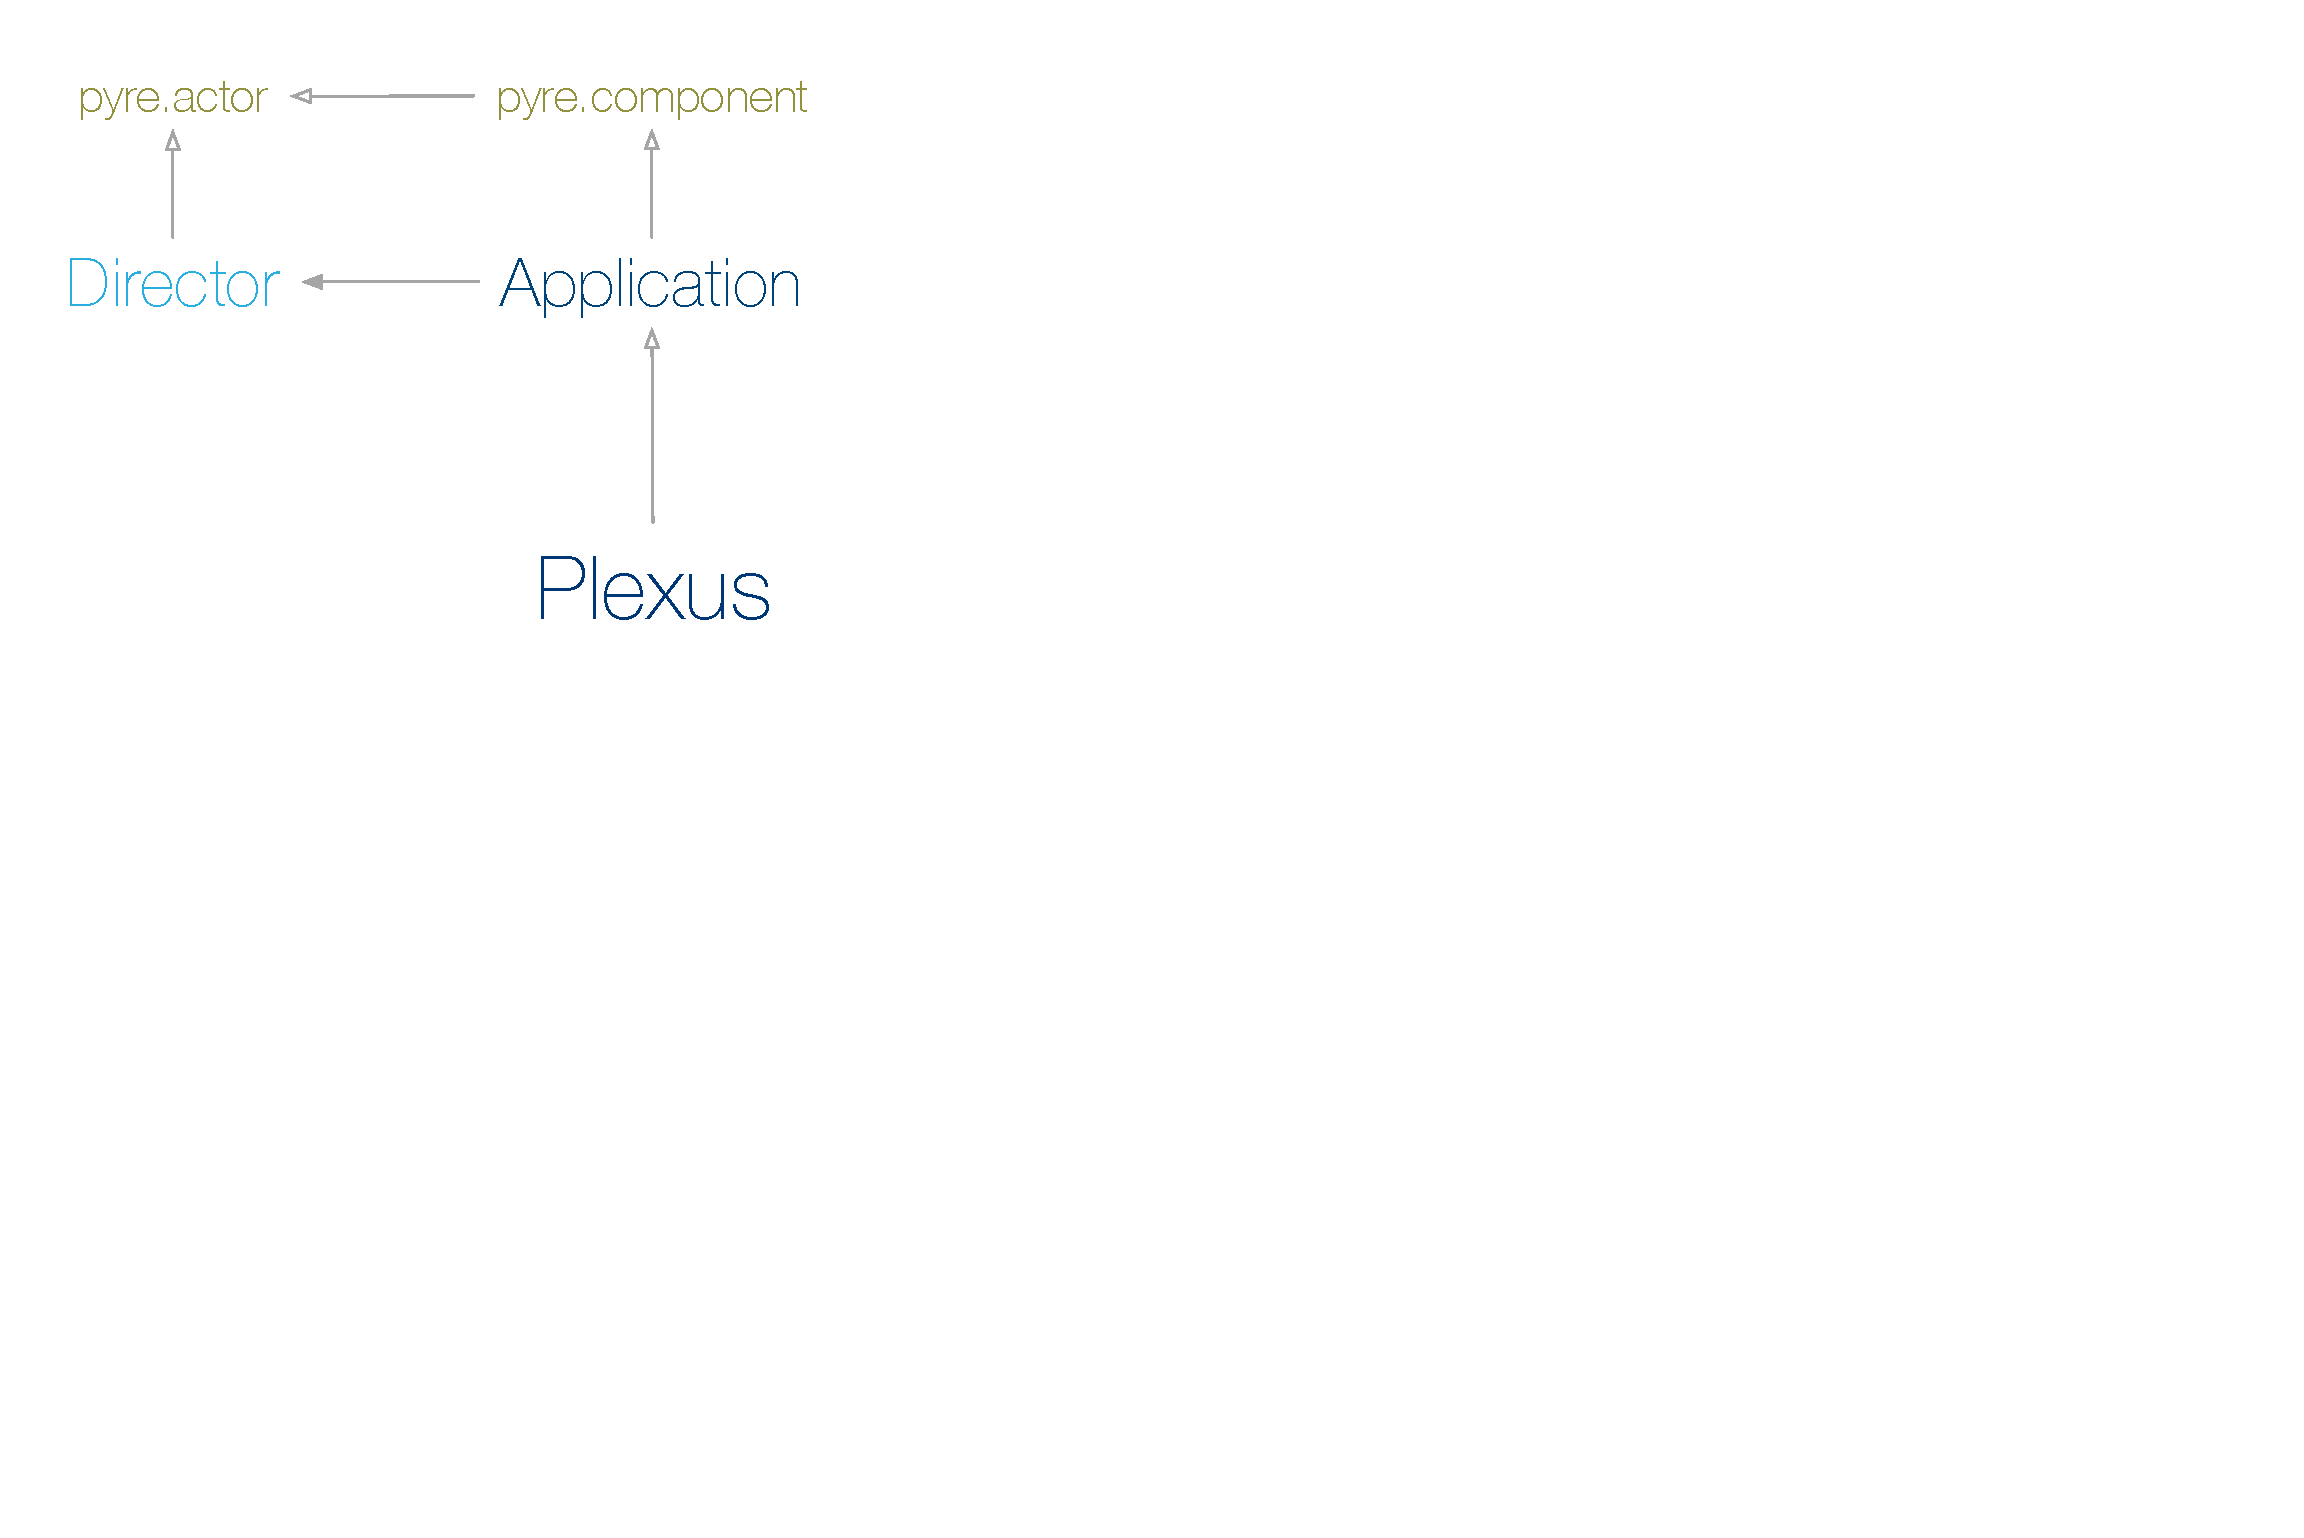
\includegraphics[width=0.9\textwidth]{pyre-plexus-pedigree}
    \end{center}
  }
  \only<3>{
    \begin{center}
      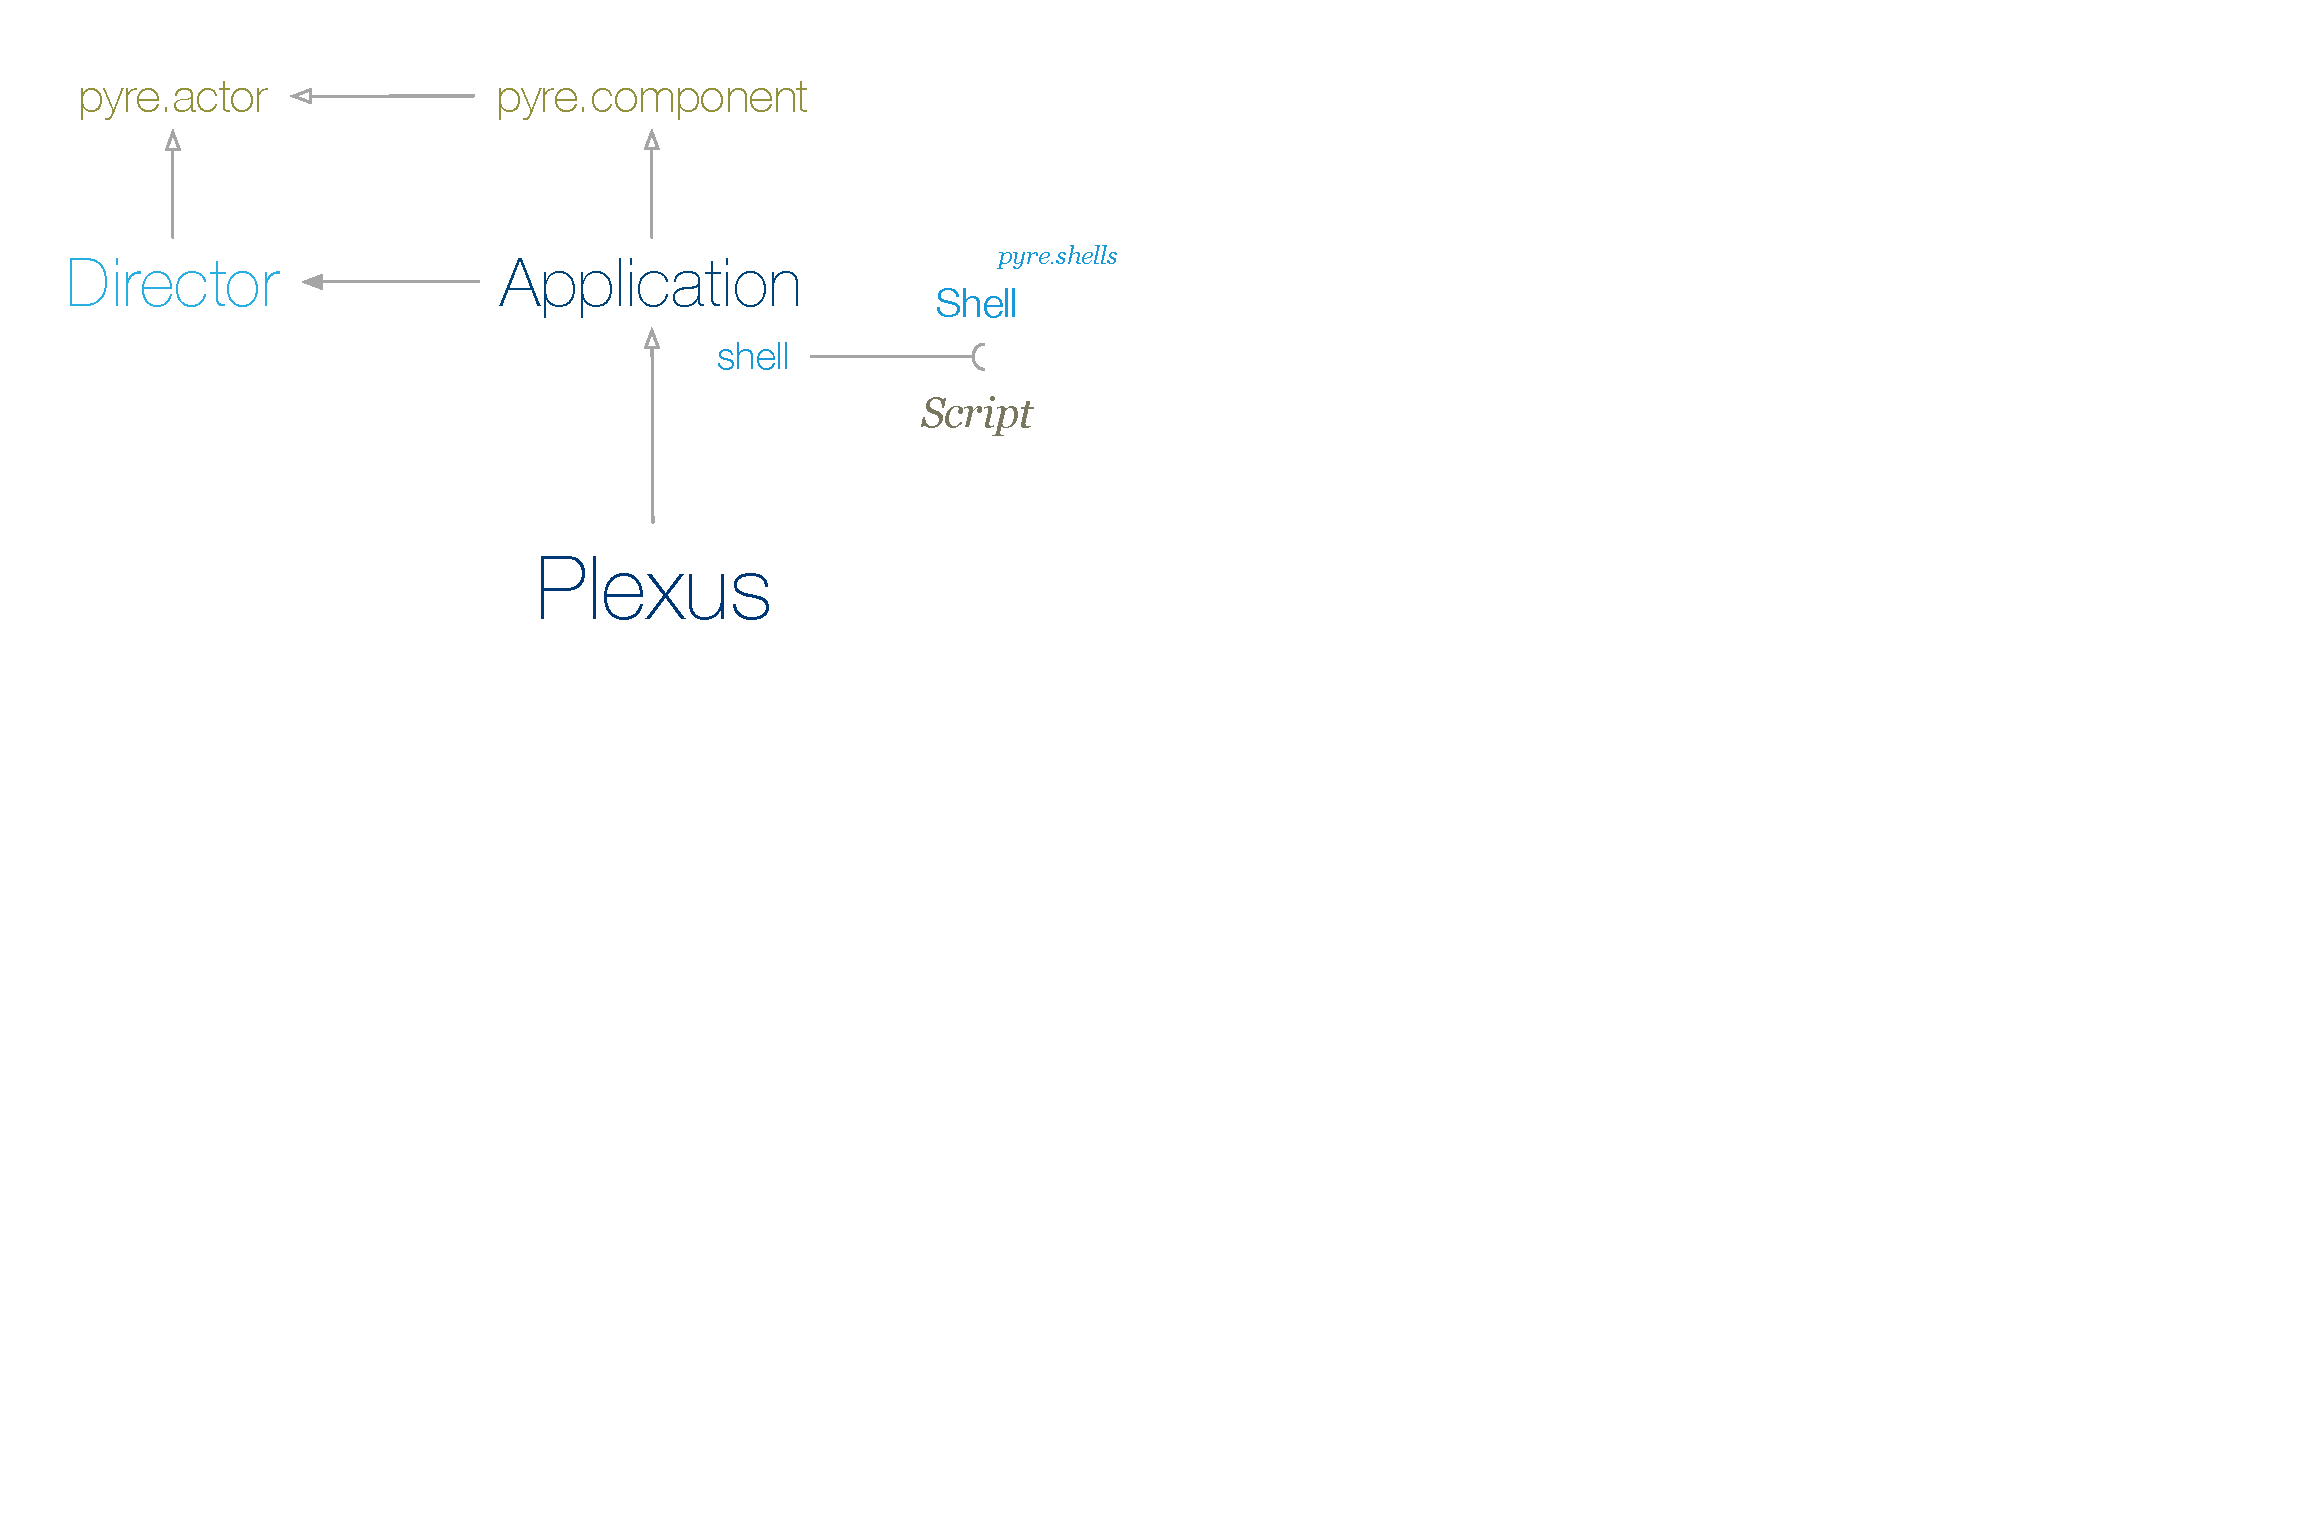
\includegraphics[width=0.9\textwidth]{pyre-plexus-traits}
    \end{center}
  }
  \only<4>{
    \begin{center}
      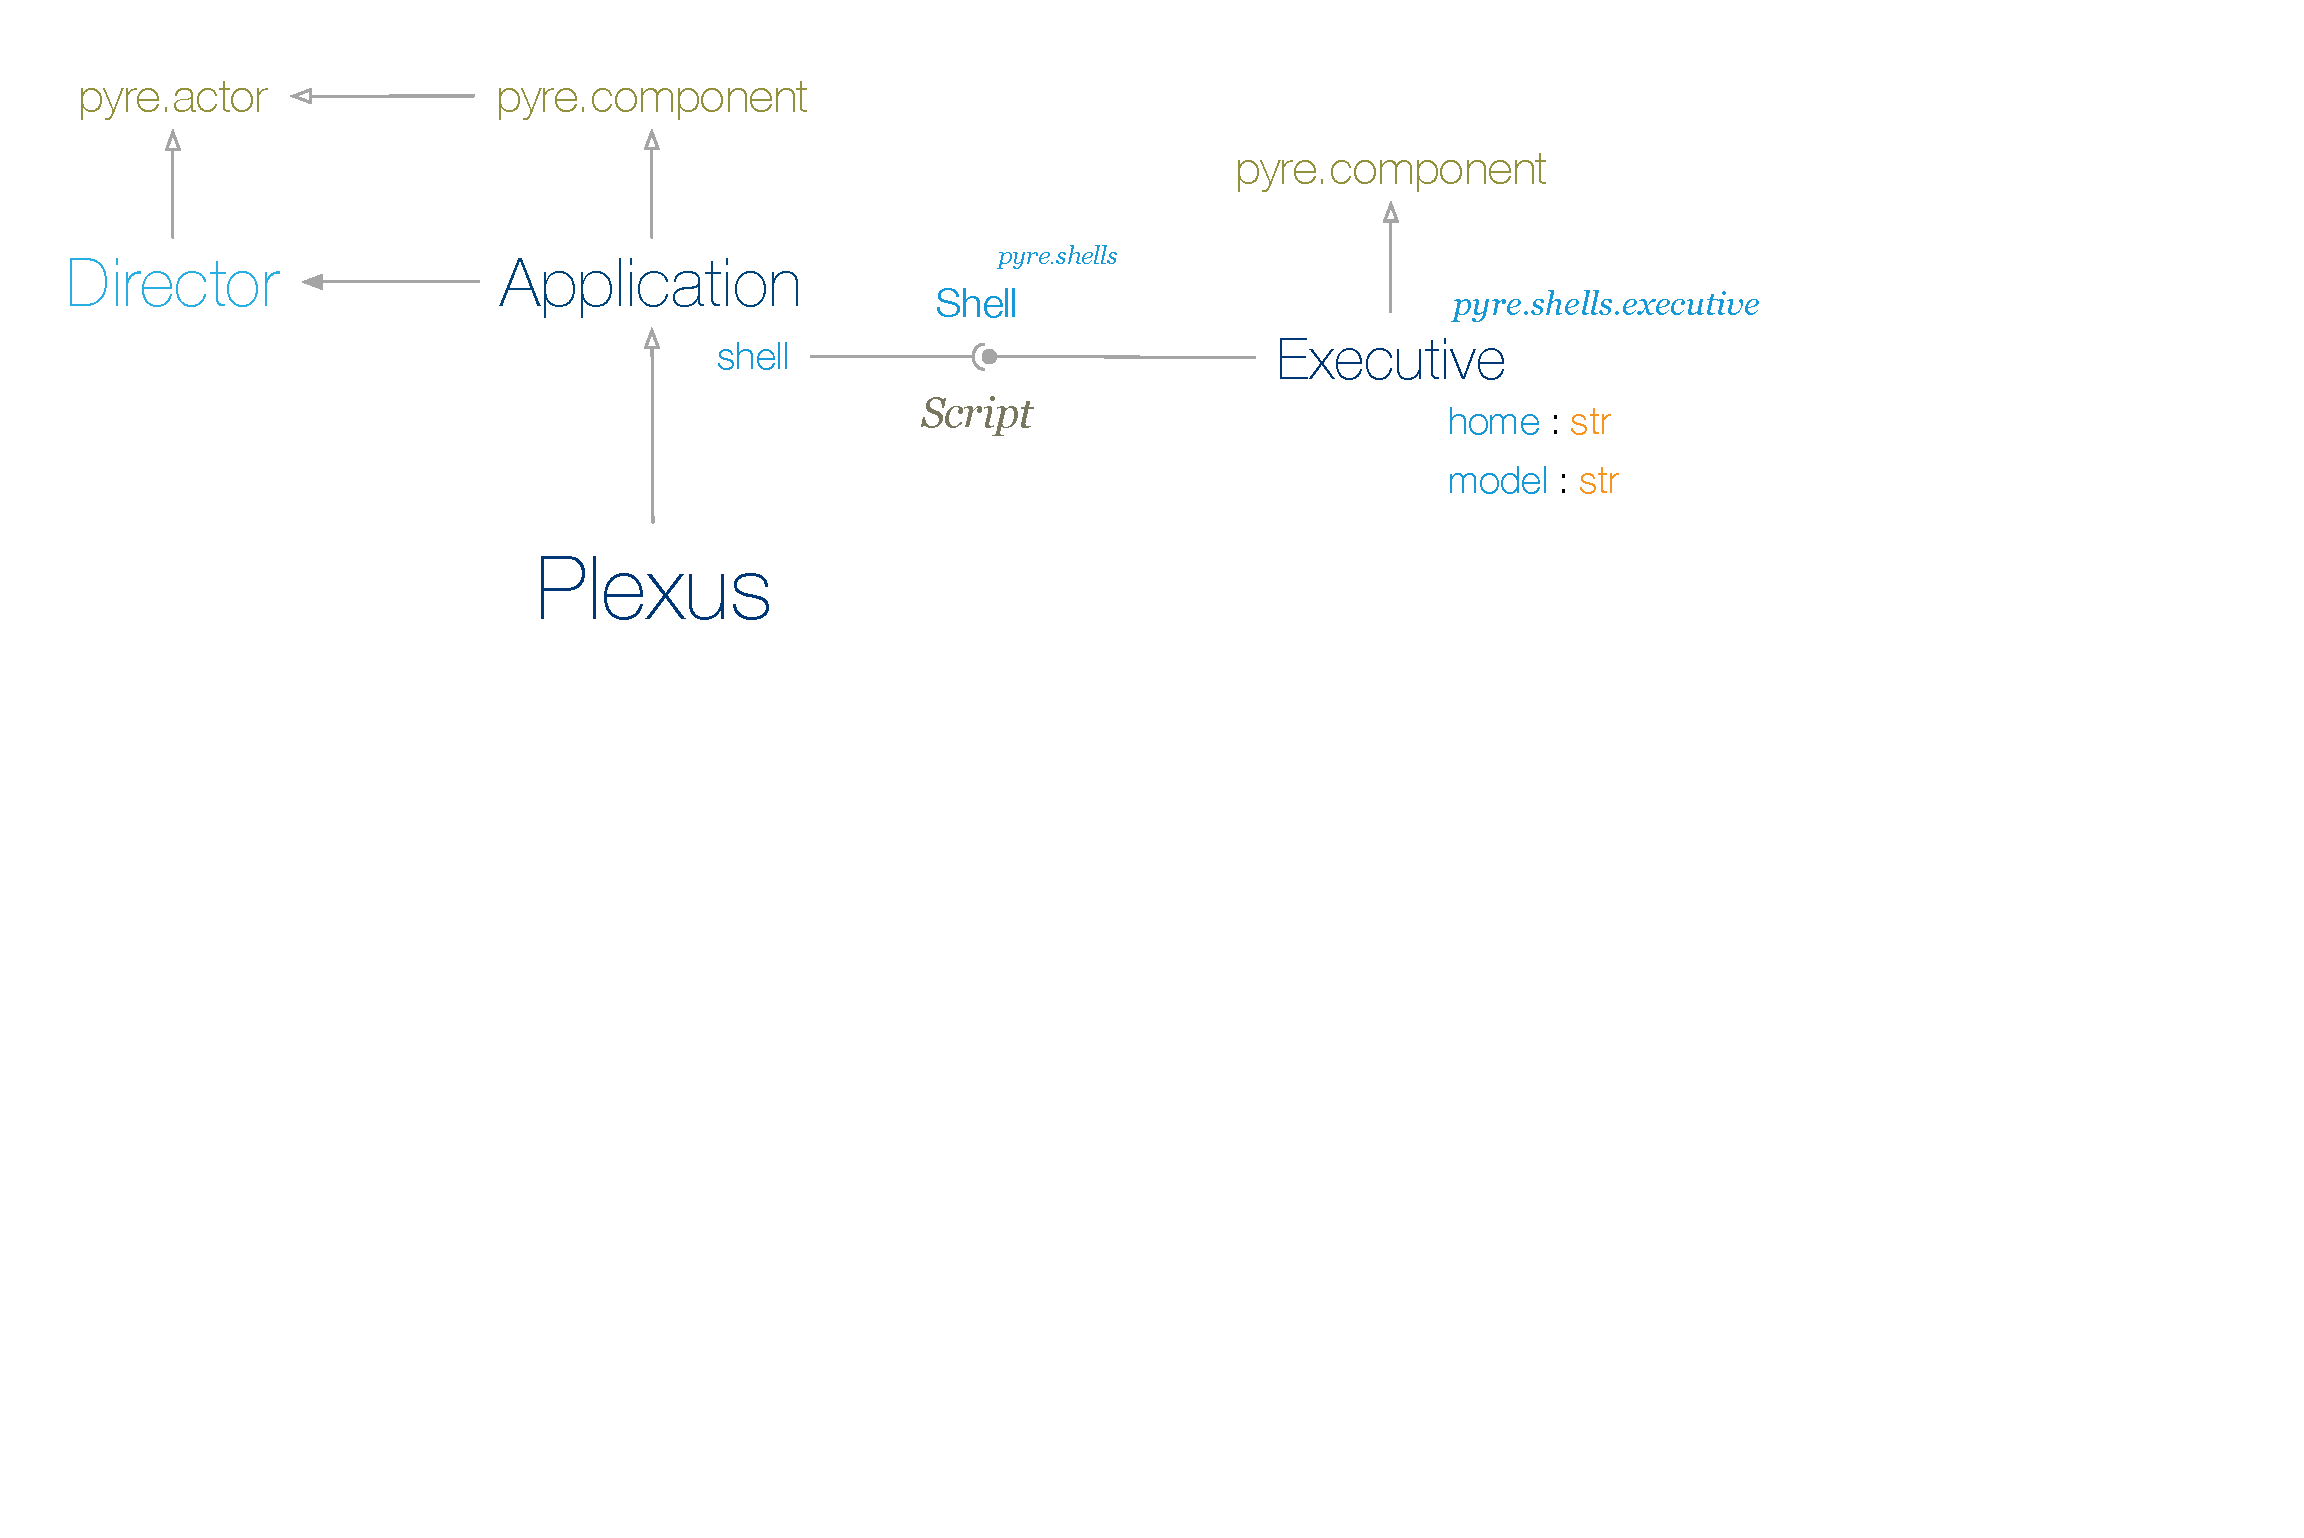
\includegraphics[width=0.9\textwidth]{pyre-plexus-executive}
    \end{center}
  }
  \only<5>{
    \begin{center}
      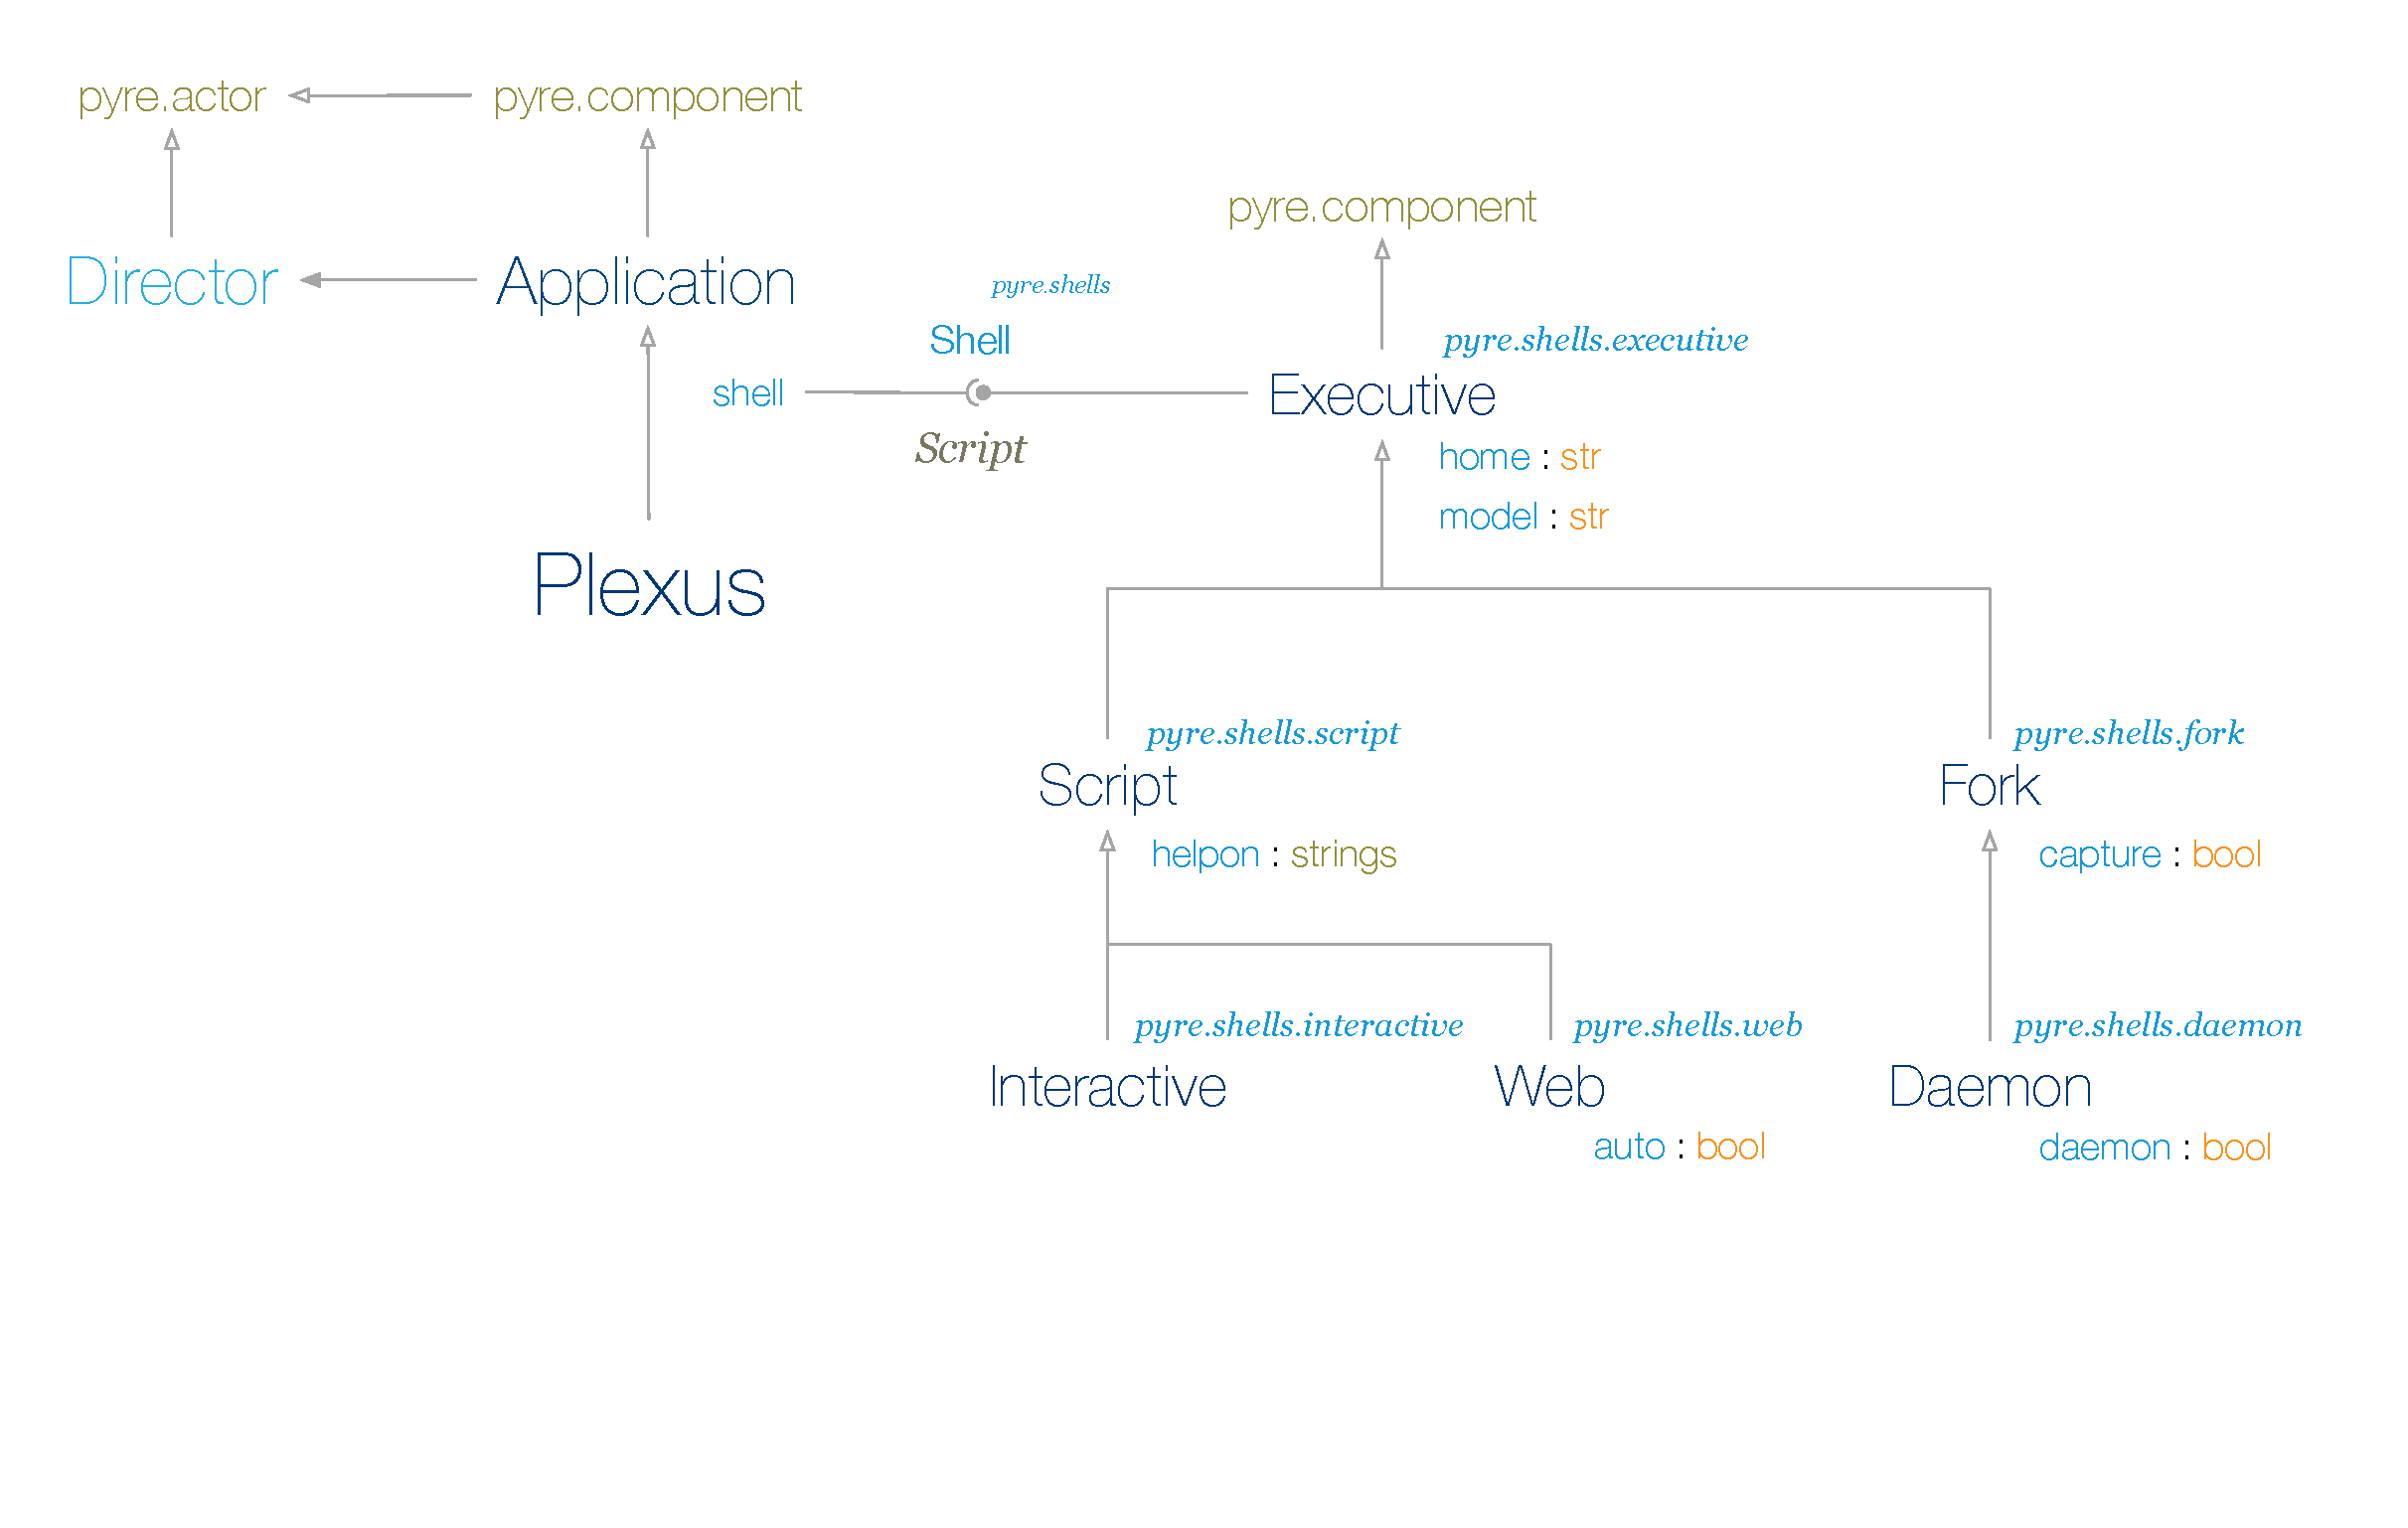
\includegraphics[width=0.9\textwidth]{pyre-plexus-shells}
    \end{center}
  }
  \only<6>{
    \begin{center}
      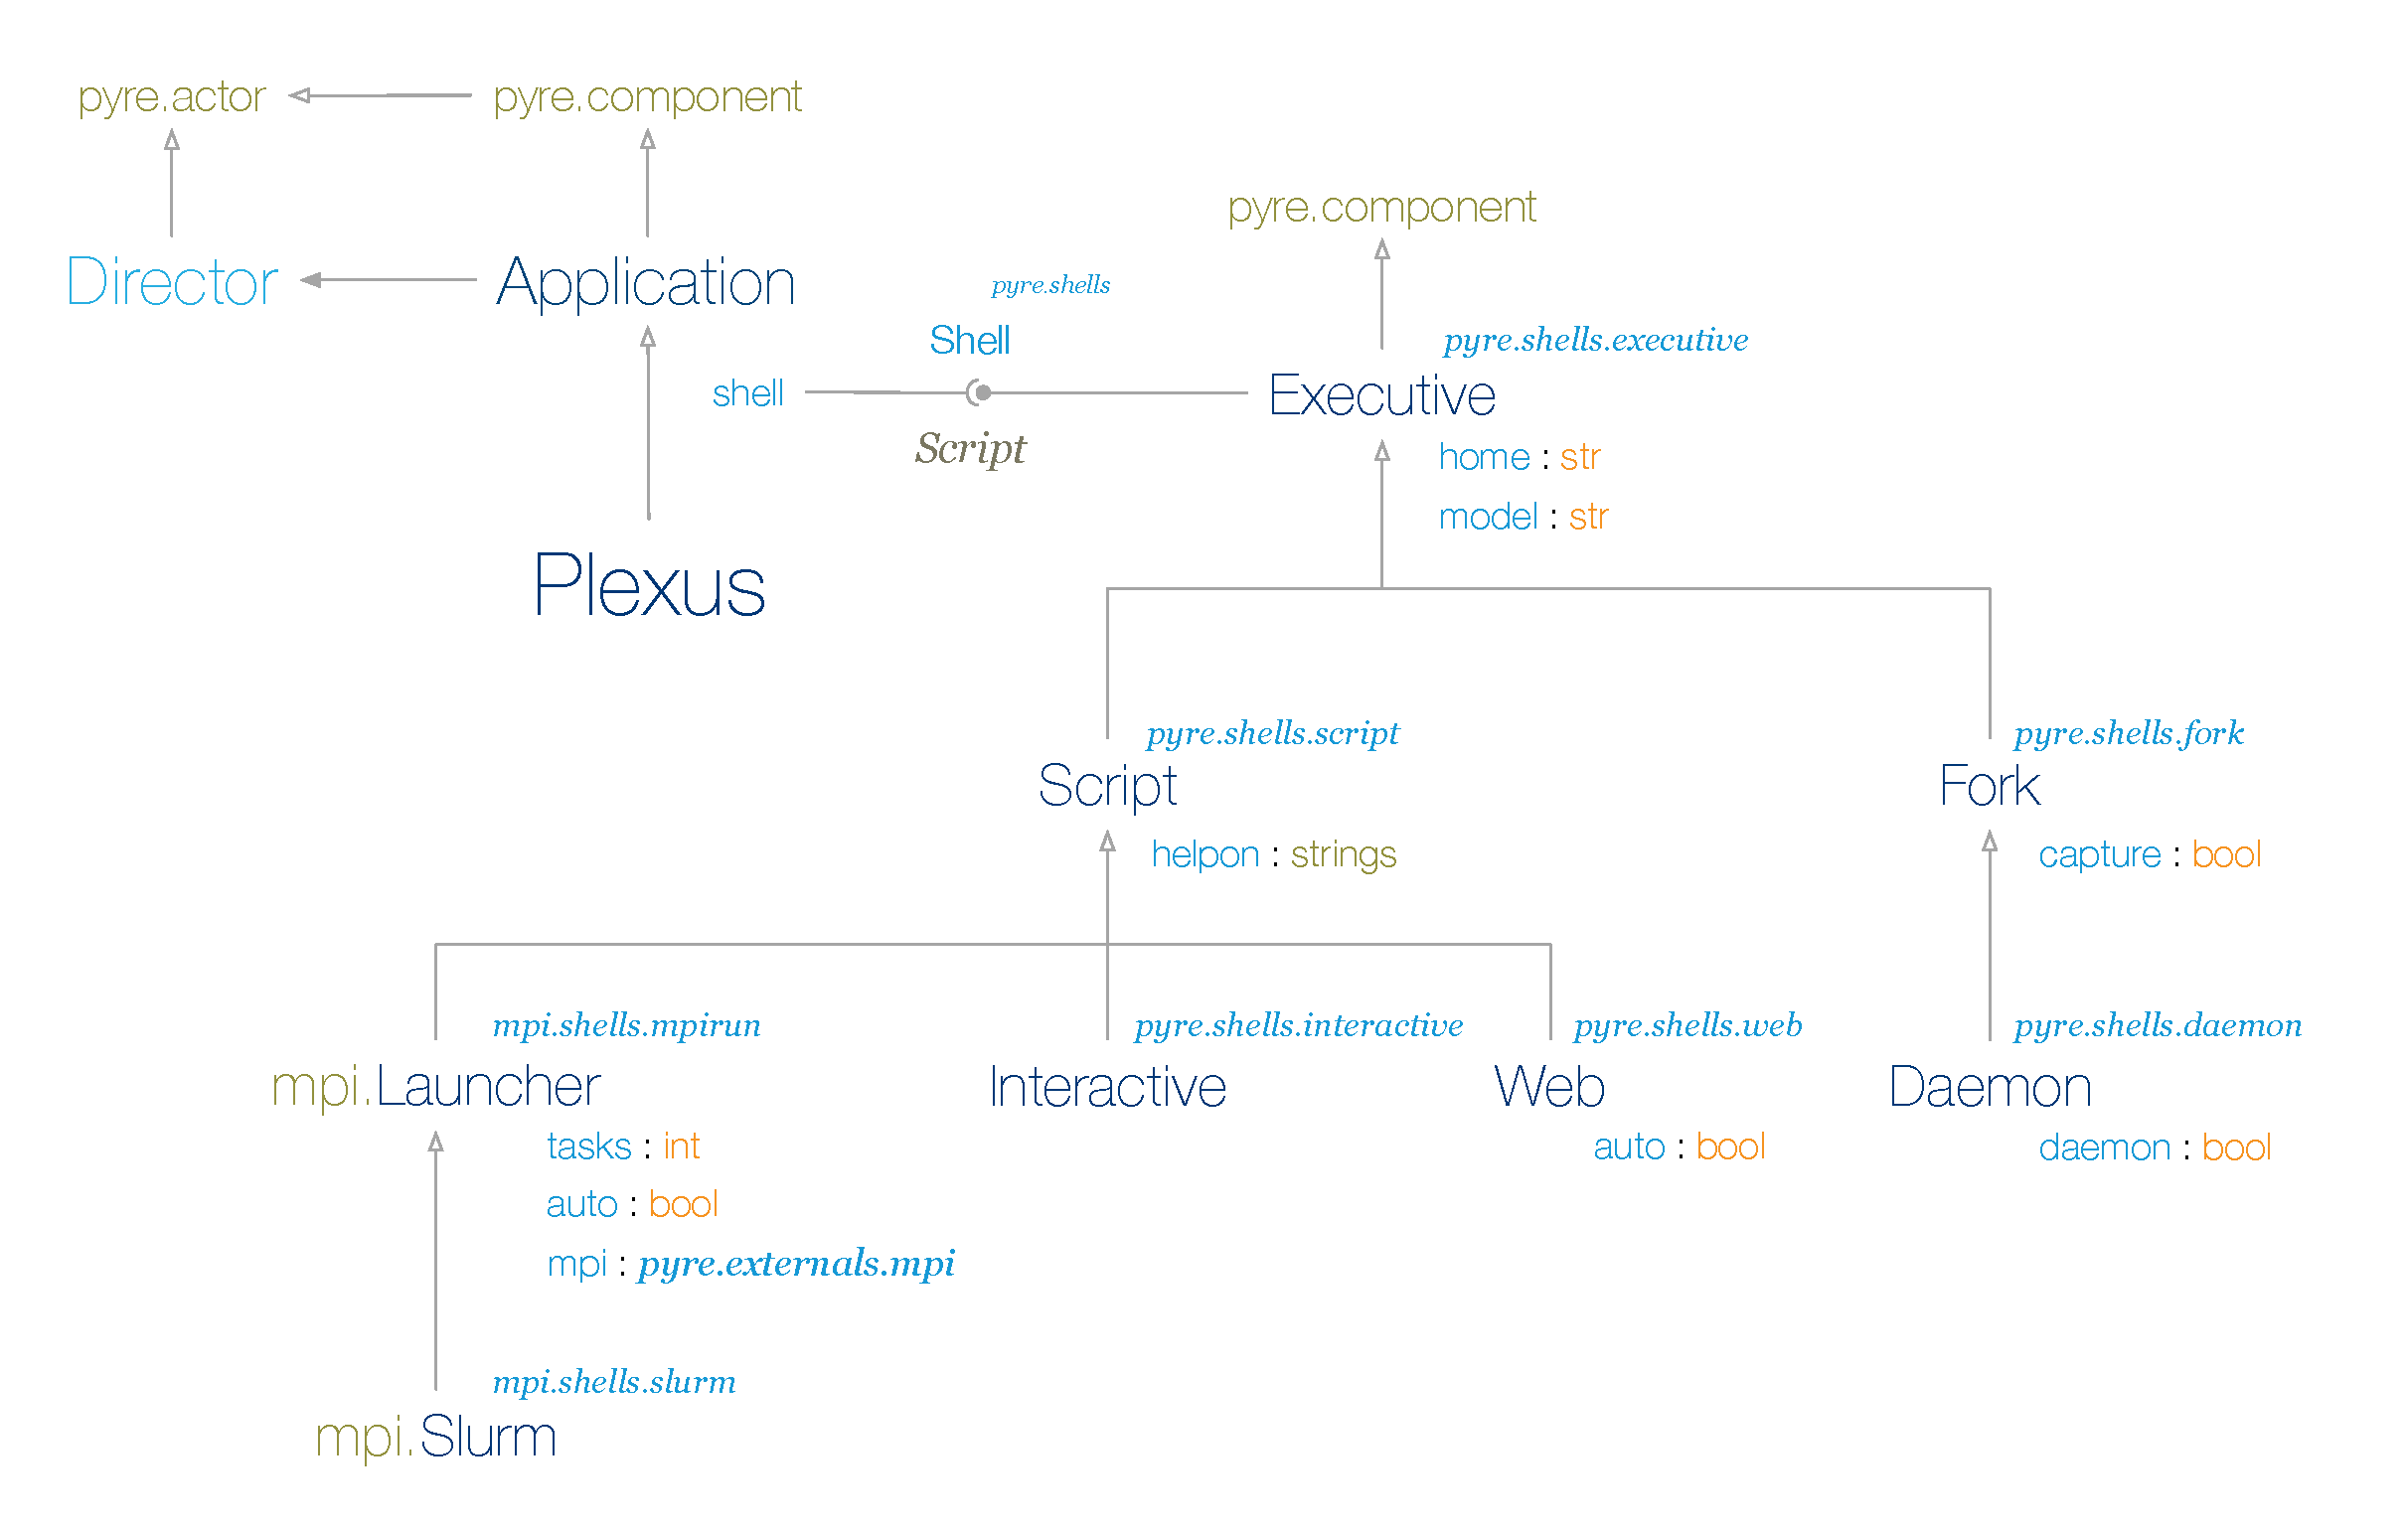
\includegraphics[width=0.9\textwidth]{pyre-plexus-mpi}
    \end{center}
  }
%
\end{frame}

% --------------------------------------

\TODO{
  \item show a simple application
    \begin{itemize}
    \item protocol as the property schema
    \end{itemize}
  \item explain plexus
  \item convert simple app into a plexus action
  \item more on configuration files
  \item private filesystems
  \item the standard layout
}


%%% Local Variables:
%%% mode: latex
%%% TeX-master: "../pyre"
%%% End:

% end of file
